%% Le lingue utilizzate, che verranno passate come opzioni al pacchetto babel. Come sempre, l'ultima indicata sar� quella primaria.
%% Se si utilizzano una o pi� lingue diverse da "italian" o "english", leggere le istruzioni in fondo.
\def\thudbabelopt{english}
%% Valori ammessi per target: bach (tesi triennale), mst (tesi magistrale), phd (tesi di dottorato).
%% --- Beamer ---
%% La chiave "beamer" attiva la modalit� slide e specifica le opzioni da passare all'omonima classe.
%% Le opzioni specificate "noamsthm,10pt" sono solamente indicative.
%% L'uso dell'opzione "ignorenonframetext" pu� creare problemi ed � quindi sconsigliato.
%% Se incontrate problemi con altre opzioni di "beamer" fatecelo sapere.
\documentclass[beamer={10pt,xcolor=dvipsnames},target=mst]{thud}

\usepackage{amsmath}
\usepackage{amssymb}
\usepackage{amsthm}
\usepackage{xcolor}
\usepackage{tikz}
\usepackage{adjustbox}
\usepackage{booktabs}
\usepackage{tabularx}
\usepackage[center]{caption}
\usepackage{mathtools}
\usepackage{stmaryrd}
\usepackage{subfig}
\usepackage{bm}


\usetikzlibrary{automata,positioning,shapes.multipart}

\makeatletter
\pgfdeclareshape{xor}
{
  \inheritsavedanchors[from=circle] 
  \inheritanchorborder[from=circle]
  \inheritanchor[from=circle]{north}
  \inheritanchor[from=circle]{north west}
  \inheritanchor[from=circle]{north east}
  \inheritanchor[from=circle]{center}
  \inheritanchor[from=circle]{west}
  \inheritanchor[from=circle]{east}
  \inheritanchor[from=circle]{mid}
  \inheritanchor[from=circle]{mid west}
  \inheritanchor[from=circle]{mid east}
  \inheritanchor[from=circle]{base}
  \inheritanchor[from=circle]{base west}
  \inheritanchor[from=circle]{base east}
  \inheritanchor[from=circle]{south}
  \inheritanchor[from=circle]{south west}
  \inheritanchor[from=circle]{south east}
  \inheritbackgroundpath[from=circle]
  \foregroundpath{
    \centerpoint%
    \pgf@xc=\pgf@x%
    \pgf@yc=\pgf@y%
    \pgfutil@tempdima=\radius%
    \pgfmathsetlength{\pgf@xb}{\pgfkeysvalueof{/pgf/outer xsep}}%  
    \pgfmathsetlength{\pgf@yb}{\pgfkeysvalueof{/pgf/outer ysep}}%  
    \ifdim\pgf@xb<\pgf@yb%
      \advance\pgfutil@tempdima by-\pgf@yb%
    \else%
      \advance\pgfutil@tempdima by-\pgf@xb%
    \fi%
    \pgfpathmoveto{\pgfpointadd{\pgfqpoint{\pgf@xc}{\pgf@yc}}{\pgfqpoint{\pgfutil@tempdima}{0pt}}}
    \pgfpathlineto{\pgfpointadd{\pgfqpoint{\pgf@xc}{\pgf@yc}}{\pgfqpoint{-\pgfutil@tempdima}{0pt}}}
    \pgfpathmoveto{\pgfpointadd{\pgfqpoint{\pgf@xc}{\pgf@yc}}{\pgfqpoint{0pt}{-\pgfutil@tempdima}}}
    \pgfpathlineto{\pgfpointadd{\pgfqpoint{\pgf@xc}{\pgf@yc}}{\pgfqpoint{0pt}{\pgfutil@tempdima}}}
    \pgfsetarrowsstart{}
    \pgfsetarrowsend{}
  }
}
\makeatother


%\usetheme{metropolis} 
\definecolor{UBCblue}{rgb}{0.04706, 0.13725, 0.46667} % UBC Blue (primary)

\usecolortheme[named=UBCblue]{structure}
\setbeamertemplate{navigation symbols}{}
\setbeamertemplate{footline}[frame number]

\setbeamerfont{bibliography item}{size=\scriptsize}
\setbeamerfont{bibliography entry author}{size=\scriptsize}
\setbeamerfont{bibliography entry title}{size=\scriptsize}
\setbeamerfont{bibliography entry location}{size=\scriptsize}
\setbeamerfont{bibliography entry note}{size=\scriptsize}

%% --- Informazioni sulla tesi ---
%% Per tutti i tipi di tesi
\title{Cryptographic Primitives for Zero-Knowledge: Theory and Implementation}
\author{Stefano Trevisani}
\course{Artificial Intelligence and Cybersecurity}
\supervisor{Dr.\ Arnab Roy}
\cosupervisor{Prof.\ Alberto Policriti\and Prof.\ Elisabeth Oswald}
\tutor{M.Sc.\ Matthias Steiner}

%% Altri campi disponibili: \tutor, \date (anno accademico, calcolato in automatico).
%% Con \supervisor, \cosupervisor e \tutor si possono indicare pi� nomi separati da \and.
%% Per le sole tesi di dottorato
%\cycle{XXVIII}
%% Campi obbligatori: \title, \author e \course.

%% Nel resto del preambolo potete personalizzare la presentazione liberamente.
%% Se incontrate problemi causati dall'interazione tra "thud" e "beamer" fatecelo sapere.

\newcommand{\range}[2]{{{#1}\dots{#2}}}
\newcommand{\overbar}[1]{\mkern 1.5mu\overline{\mkern-1.5mu#1\mkern-1.5mu}\mkern 1.5mu} %chktex 1

\makeatletter
\newcommand*{\transpose}{{\mathpalette\@transpose{}}} %chktex 21
\newcommand*{\@transpose}[2]{\raisebox{\depth}{\(\m@th#1\intercal \)}}

\DeclarePairedDelimiter{\Pipes}{\lvert}{\rvert}
\DeclarePairedDelimiter{\Angular}{\langle}{\rangle}
\DeclarePairedDelimiter{\Braces}{\{}{\}} %chktex 21
\DeclarePairedDelimiter{\Brackets}{[}{]} %chktex 9
\DeclarePairedDelimiter{\Parens}{(}{)}   %chktex 9

\newcommand{\Set}[1]{\Braces*{#1}}
\newcommand{\Tuple}[1]{\Parens*{#1}}
\newcommand{\Encode}[1]{\Angular*{#1}}
\newcommand{\call}[2]{#1\Parens*{#2}}
\newcommand{\extend}[2]{#1\Brackets*{#2}}
\newcommand{\abs}[1]{\Pipes*{#1}}
\newcommand{\explicit}[1]{\widehat{#1}}
\newcommand{\id}{\mathrm{e}}
\newcommand{\inv}[1]{\overbar{#1}}
\newcommand{\fooid}{\mathrm{id}}
\newcommand{\gengroup}[1]{\left\langle#1\right\rangle}
\newcommand{\bitand}{\mathbin{\textnormal{\textsc{and}}}}
\newcommand{\bitxor}{\mathbin{\textnormal{\textsc{xor}}}}
\newcommand{\Endset}[1]{\mathrm{End}\left(#1\right)}


\newcommand{\BigO}[1]{\call{\mathcal{O}}{#1}}
\newcommand{\SmallO}[1]{\call{o}{#1}}
\newcommand{\BigOmega}[1]{\call{\Omega}{#1}}
\newcommand{\SmallOmega}[1]{\call{\omega}{#1}}
\newcommand{\BigTheta}[1]{\call{\Theta}{#1}}
\newcommand{\Complexity}{\mathsf{C}}
\newcommand{\Time}{\mathsf{T}}
\newcommand{\Space}{\mathsf{S}}


\newcommand{\then}{\Rightarrow}

\newcommand{\Ptime}{\textnormal{\textsc{P}}}
\newcommand{\NPtime}{\textnormal{\textsc{NP}}}
\newcommand{\NPcomplete}{\textnormal{\textsc{NP-complete}}}

\newcommand{\Stamp}{\texttt{Stamp}}
\newcommand{\Blocc}{\texttt{Blocc}}

\newcommand{\Tape}{\mathfrak{T}}
\newcommand{\Tapework}{\mathfrak{W}}
\newcommand{\Tapein}{\mathfrak{I}}
\newcommand{\Tapeout}{\mathfrak{O}}
\newcommand{\Taperand}{\mathfrak{P}}
\newcommand{\Tapesend}{\mathfrak{S}}
\newcommand{\Taperec}{\mathfrak{R}}

\newcommand{\maybeequals}{\mathrel{\overset{?}{=}}}


\begin{document}

%% Il frontespizio prima di tutto!
%% \maketitle accetta gli stessi argomenti opzionali di \begin{frame} (p.es. "[plain]")
\maketitle

%% Diapositiva
\begin{frame}{Interactive Proof Systems~\cite{GoldwasserMR1989}}
  \begin{figure}
    \centering
    \adjustbox{max height=96pt,keepaspectratio}
    {
    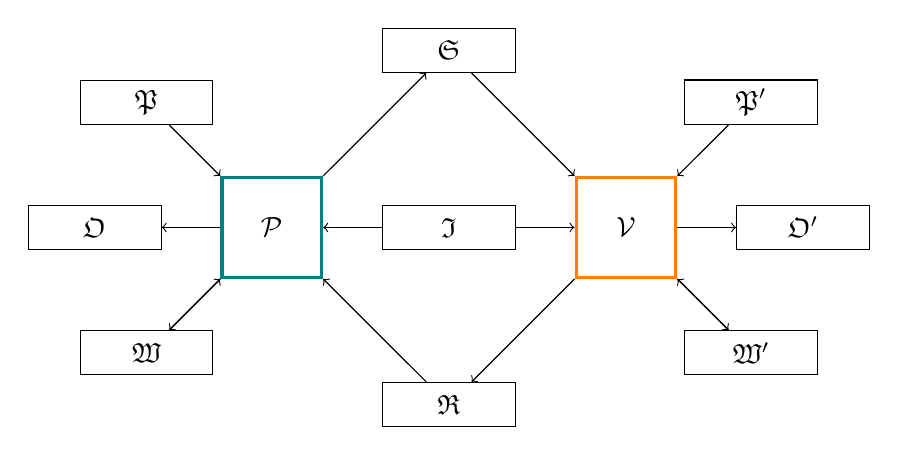
\begin{tikzpicture}[node distance=64pt,on grid,auto]
      \node[state,shape=rectangle,minimum height=16pt, minimum width=48pt] (in)  {\(\Tapein \)};
      \node[state,shape=rectangle,very thick,draw=teal,minimum size=36pt,left =of in]   (m0)         {\(\mathcal{P}\)};
      \node[state,shape=rectangle,very thick,draw=orange,minimum size=36pt,right =of in] (m1)  {\(\mathcal{V}\)};
      \node[state,shape=rectangle,minimum height=16pt, minimum width=48pt,above left =of m0] (p0)  {\(\Taperand \)};
      \node[state,shape=rectangle,minimum height=16pt, minimum width=48pt,above right =of m1] (p1)  {\(\Taperand' \)};
      \node[state,shape=rectangle,minimum height=16pt, minimum width=48pt,below left =of m0] (w0)  {\(\Tapework \)};
      \node[state,shape=rectangle,minimum height=16pt, minimum width=48pt,below right =of m1] (w1)  {\(\Tapework' \)};
      \node[state,shape=rectangle,minimum height=16pt, minimum width=48pt,above =of in] (s0)  {\(\Tapesend \)};
      \node[state,shape=rectangle,minimum height=16pt, minimum width=48pt,below =of in] (r0)  {\(\Taperec \)};
      \node[state,shape=rectangle,minimum height=16pt, minimum width=48pt,left =of m0] (o0)  {\(\Tapeout \)};
      \node[state,shape=rectangle,minimum height=16pt, minimum width=48pt,right =of m1] (o1)  {\(\Tapeout' \)};
      \path[->]
      (in) edge (m0)
      (in) edge (m1)
      (p0) edge (m0)
      (p1) edge (m1)
      (w0) edge (m0)
      (m0) edge (w0)
      (w1) edge (m1)
      (m1) edge (w1)
      (m0) edge (s0)
      (s0) edge (m1)
      (m1) edge (r0)
      (r0) edge (m0)
      (m0) edge (o0)
      (m1) edge (o1)
      ;
    \end{tikzpicture}
    }
  \end{figure}
  \begin{itemize}
    \item \textcolor{teal}{Prover}: wants to prove a statement by creating a proof.
    \item \textcolor{orange}{Verifier}: wants to check the soundness of the proof.
    \item Modeled as \emph{interactive I/O probabilistic Turing machines}.
    \item \textcolor{orange}{Verifier} is polynomially bounded.
    \item \textcolor{orange}{Verifier} might be fooled with \emph{negligible} probability.
    \item \textsc{IP} = \textsc{PSPACE}~\cite{Shamir1992}.
  \end{itemize}
\end{frame}

\begin{frame}{Verifiable Computation}
  \begin{figure}
    \centering
    \href{https://www.template.net/editable/illustrations}{
      
\includegraphics[scale=0.0625]{res/cloud_computing.pdf}}
  \end{figure}
  Proof systems can be used for \emph{verifiable computation}:
  \begin{itemize}
    \item Delegating heavy loads to the cloud~\cite{AndersonCKLW2002}.
    \item Calculate household due bills~\cite{ParnoGHR2013}.
    \item \textbf{Verifying transactions on the blockchain.}~\cite{SassonCGGMTV2014}
  \end{itemize}
\end{frame}

\begin{frame}{ZK-SNARK systems}
  \begin{figure}
    \centering
      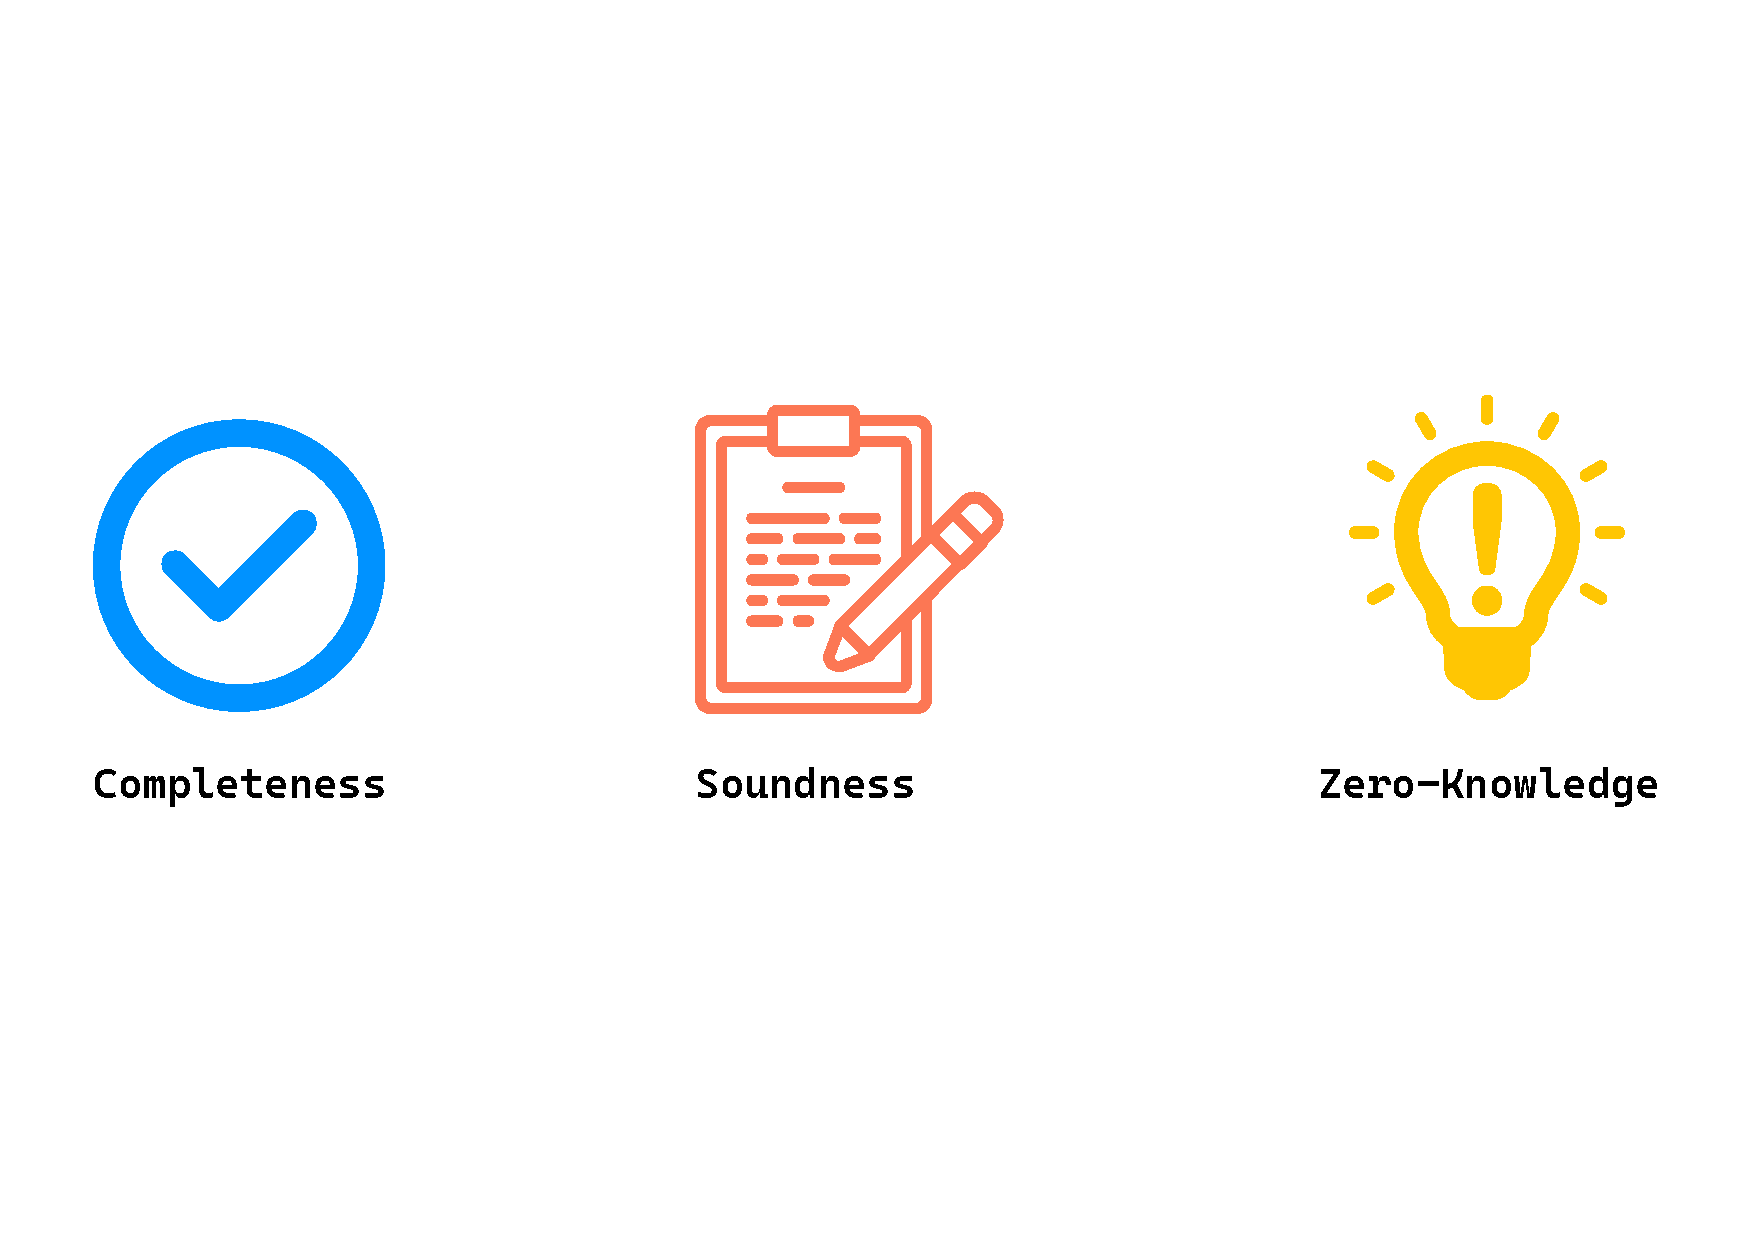
\includegraphics[scale=0.25]{res/Zero-Knowledge-Proofs-Properties.pdf}
  \end{figure}
  ZK-SNARK systems:
  \begin{itemize}
    \item \textcolor{teal}{Prover} might be \textbf{dishonest} \(\implies \) proof system.
    \item \textcolor{orange}{Verifier} might be \textbf{curious} \(\implies \) \emph{Zero-Knowledge}.
    \item Verification must be fast \(\implies \) \emph{Succinct}.
    \item There may be many verifiers  \(\implies \) \emph{Non-interactive}.
    \item \textcolor{teal}{Prover} is polynomially bounded \(\implies \) \emph{Argument of Knowledge}.
  \end{itemize}
\end{frame}

\begin{frame}{SNARKs via QAPs~\cite{GennaroGPR2012,ParnoGHR2013,Groth2016}}
  \begin{figure}
    \centering
      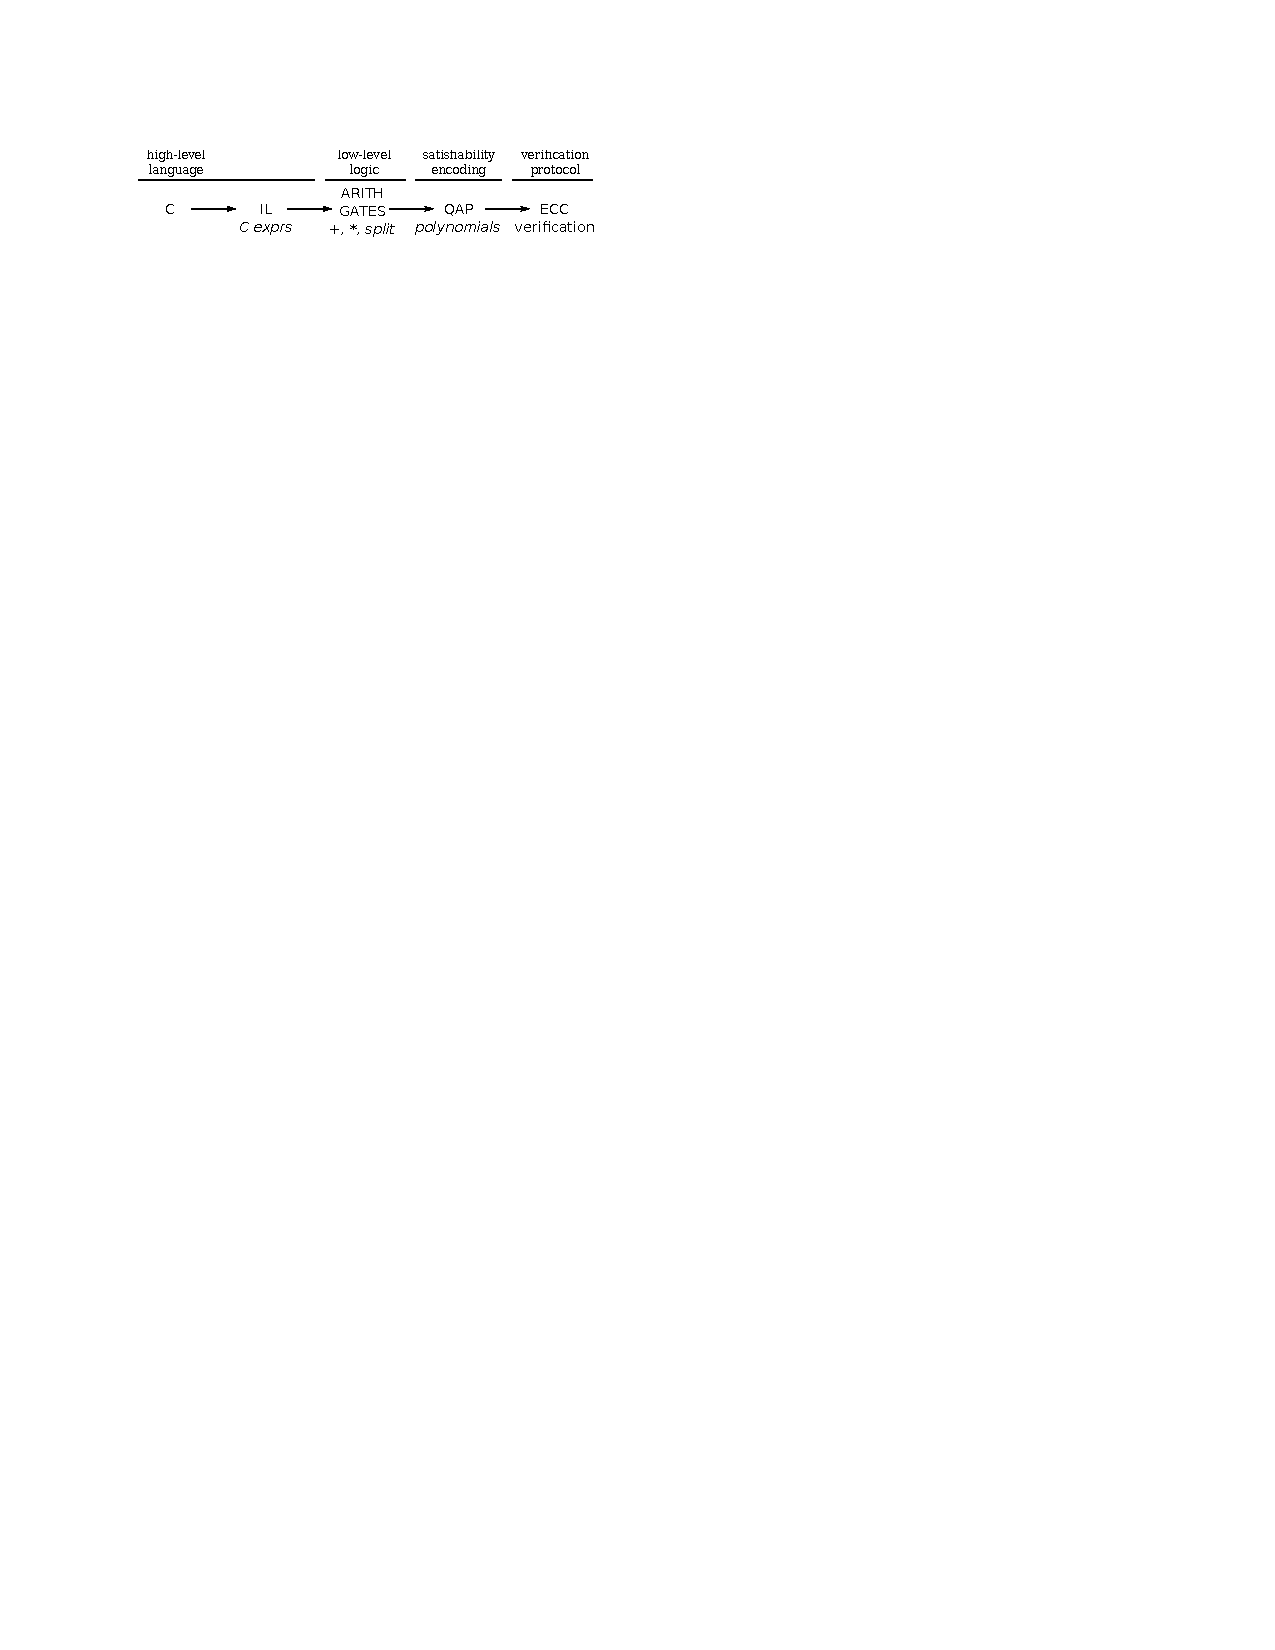
\includegraphics{res/pinocchio.pdf}
  \end{figure}
  Setting up a SNARK for some computable function:
  \begin{enumerate}
    \item Bounded computations represented through \emph{arithmetic circuits}.
    \item \emph{Rank-1 constraint systems (R1CSs)} encode circuit invariants.
    \item \emph{Quadratic Arithmetic Programs (QAPs)} ``compress'' R1CSs.
    \item \emph{Private key} to build the proof, \emph{public key} to verify it.
    \item Exploit \emph{bilinear maps}, work in the exponent: discrete \(\log \) is hard!
    \item Inject random noise for statistical zero-knowledge.
  \end{enumerate}
  \vspace*{16pt}
  Generating the keys incurs into the \emph{toxic waste} problem\dots
\end{frame}

\begin{frame}{The Blockchain}
  \begin{figure}
    \centering
    \adjustbox{max height=128pt,keepaspectratio}{
    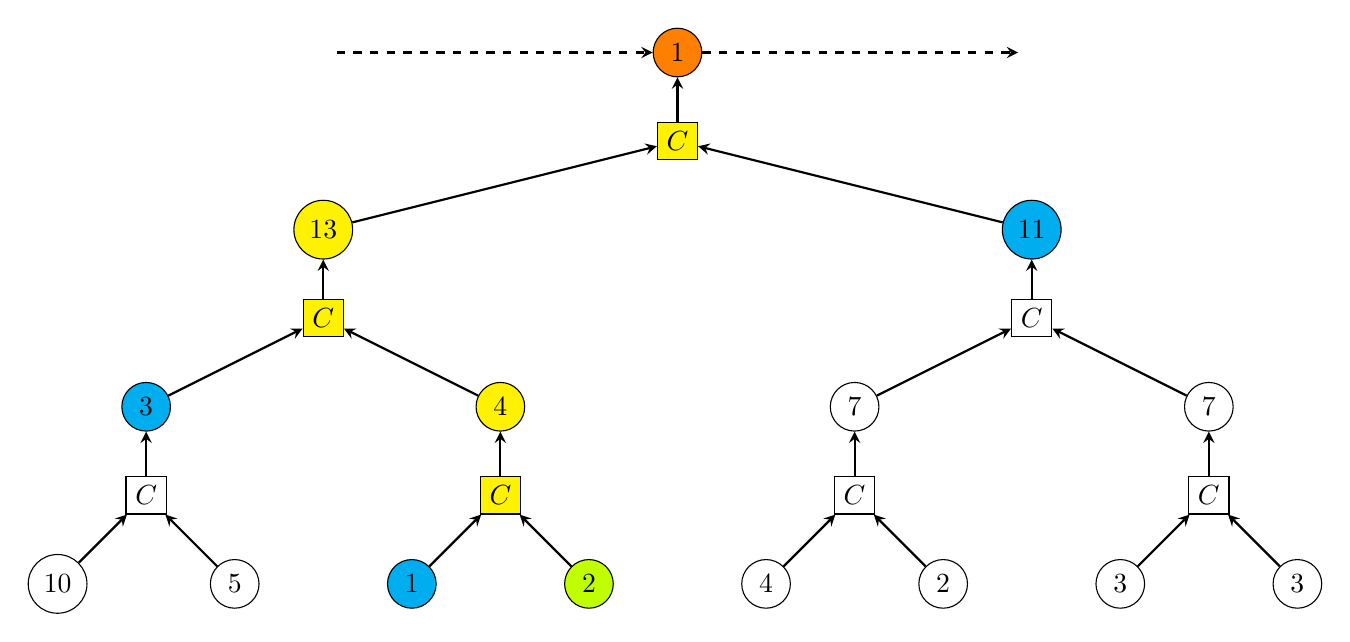
\begin{tikzpicture}[node distance={32pt}, node/.style = {draw, circle},on grid=true]
      \node[node] (y1) {\(10\)};
      \node[node,draw=none] (m1) [right of=y1] {};
      \node[node] (y2) [right of=m1] {\(5\)};
      \node[node,draw=none] (m2) [right of=y2] {};
      \node[node,fill=cyan] (y3) [right of=m2] {\(1\)};
      \node[node,draw=none] (m3) [right of=y3] {};
      \node[node,fill=lime] (y4) [right of=m3] {\(2\)};
      \node[node,draw=none] (m4) [right of=y4] {};
      \node[node] (y5) [right of=m4] {\(4\)};
      \node[node,draw=none] (m5) [right of=y5] {};
      \node[node] (y6) [right of=m5] {\(2\)};
      \node[node,draw=none] (m6) [right of=y6] {};
      \node[node] (y7) [right of=m6] {\(3\)};
      \node[node,draw=none] (m7) [right of=y7] {};
      \node[node] (y8) [right of=m7] {\(3\)};

      \node[node,shape=rectangle] (d1) [above of=m1] {\(C\)};
      \node[node,draw=none] (m8) [above of=m2] {};
      \node[node,shape=rectangle,fill=yellow] (d2) [above of=m3] {\(C\)};
      \node[node,draw=none] (m9) [above of=m4] {};
      \node[node,shape=rectangle] (d3) [above of=m5] {\(C\)};
      \node[node,draw=none] (m10) [above of=m6] {};
      \node[node,shape=rectangle] (d4) [above of=m7] {\(C\)};

      \node[node,fill=cyan] (x1) [above of=d1] {\(3\)};
      \node[node,draw=none] (n1) [above of=m8] {};
      \node[node,fill=yellow] (x2) [above of=d2] {\(4\)};
      \node[node,draw=none] (n2) [above of=m9] {};
      \node[node] (x3) [above of=d3] {\(7\)};
      \node[node,draw=none] (n3) [above of=m10] {};
      \node[node] (x4) [above of=d4] {\(7\)};
      \node[node,shape=rectangle,fill=yellow] (c1) [above of=n1] {\(C\)};
      \node[node,shape=rectangle] (c2) [above of=n3] {\(C\)};

      \node[node,fill=yellow] (x5) [above of=c1] {\(13\)};
      \node[node,draw=none] (n3) [above of=n2] {};
      \node[node,draw=none] (n4) [above of=n3] {};
      \node[node,fill=cyan] (x6) [above of=c2] {\(11\)};
      \node[node,shape=rectangle,fill=yellow] (c3) [above of=n4] {\(C\)};

      \node[node,fill=orange] (x7) [above of=c3] {\(1\)};
      \node[node,draw=none] (n5) [left =128pt of x7] {};
      \node[node,draw=none] (n6) [right =128pt of x7] {};


      \draw[-stealth,thick] (y1) to (d1);
      \draw[-stealth,thick] (y2) to (d1);
      \draw[-stealth,thick] (y3) to (d2);
      \draw[-stealth,thick] (y4) to (d2);
      \draw[-stealth,thick] (y5) to (d3);
      \draw[-stealth,thick] (y6) to (d3);
      \draw[-stealth,thick] (y7) to (d4);
      \draw[-stealth,thick] (y8) to (d4);

      \draw[-stealth,thick] (d1) to (x1);
      \draw[-stealth,thick] (d2) to (x2);
      \draw[-stealth,thick] (d3) to (x3);
      \draw[-stealth,thick] (d4) to (x4);


      \draw[-stealth,thick] (x1) to (c1);
      \draw[-stealth,thick] (x2) to (c1);
      \draw[-stealth,thick] (x3) to (c2);
      \draw[-stealth,thick] (x4) to (c2);

      \draw[-stealth,thick] (c1) to (x5);
      \draw[-stealth,thick] (c2) to (x6);

      \draw[-stealth,thick] (x5) to (c3);
      \draw[-stealth,thick] (x6) to (c3);

      \draw[-stealth,thick] (c3) to (x7);

      \draw[dashed,-stealth,thick] (n5) to (x7);
      \draw[dashed,-stealth,thick] (x7) to (n6);
    \end{tikzpicture}
    }
  \end{figure}
  \begin{itemize}
    \item Groups of transactions are leaves of a \emph{Merkle tree}~\cite{Merkle1988}.
    \item Bottom-up computation using a \textbf{compression function}.
    \item The root contains the \emph{commitment} (among other data).
    \item Verify a commitment following the \emph{authentication path}.
  \end{itemize}
\end{frame}

\begin{frame}{Cryptographic Compression Functions}
  \begin{figure}
    \centering
    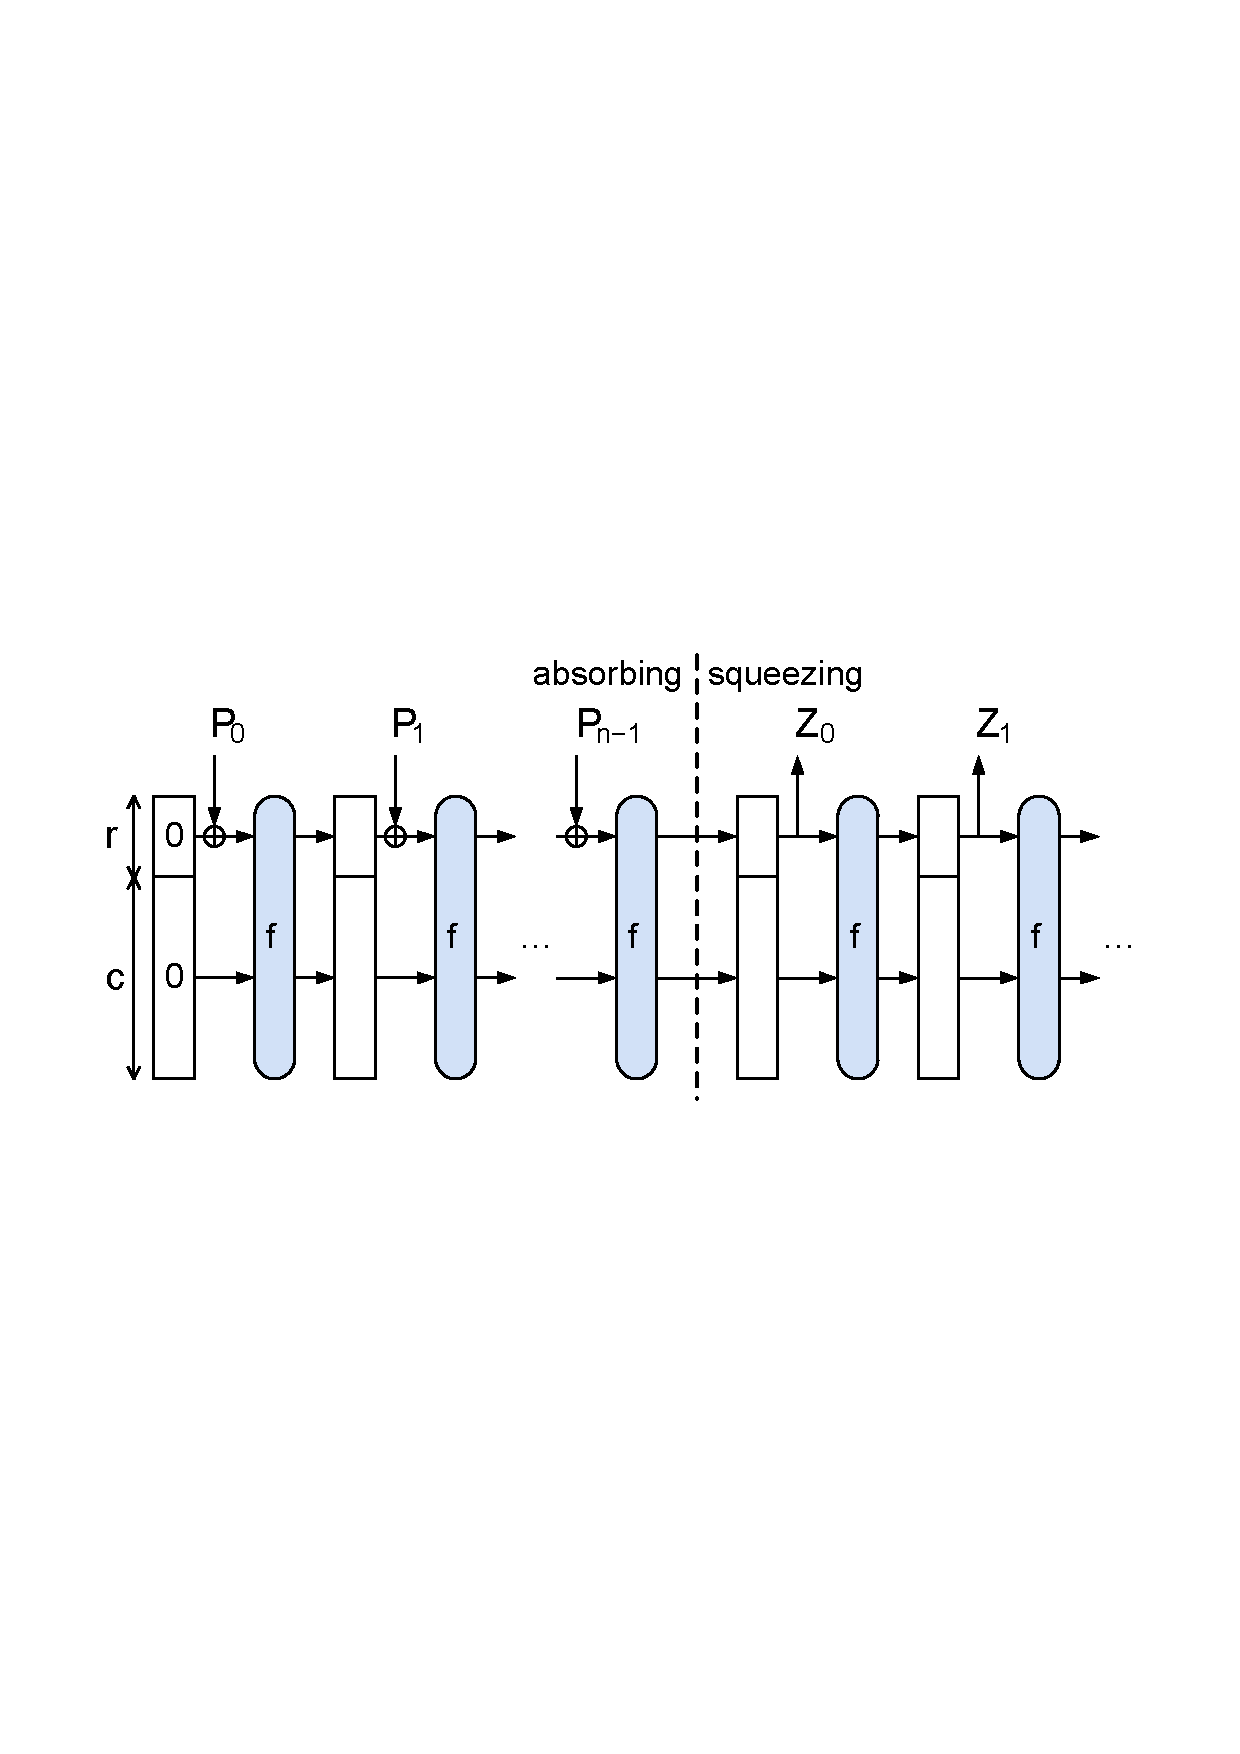
\includegraphics[scale=0.5]{res/SpongeConstruction.pdf}
  \end{figure}
  One-way compression functions (OWCF):
  \begin{itemize}
    \item Many inputs reduced to a few outputs (e.g.\  \(2\)-to-\(1\)).
    \item Easy to compute, but hard to invert and find collisions.
    \item Usually derived from one-way permutations.
    \item Constructed through secure schemes, like Sponge~\cite{BertoniDPA2007}.
  \end{itemize}
\end{frame}

\begin{frame}{SHA~\cite{Dang2015}}
  \begin{figure}
    \centering
    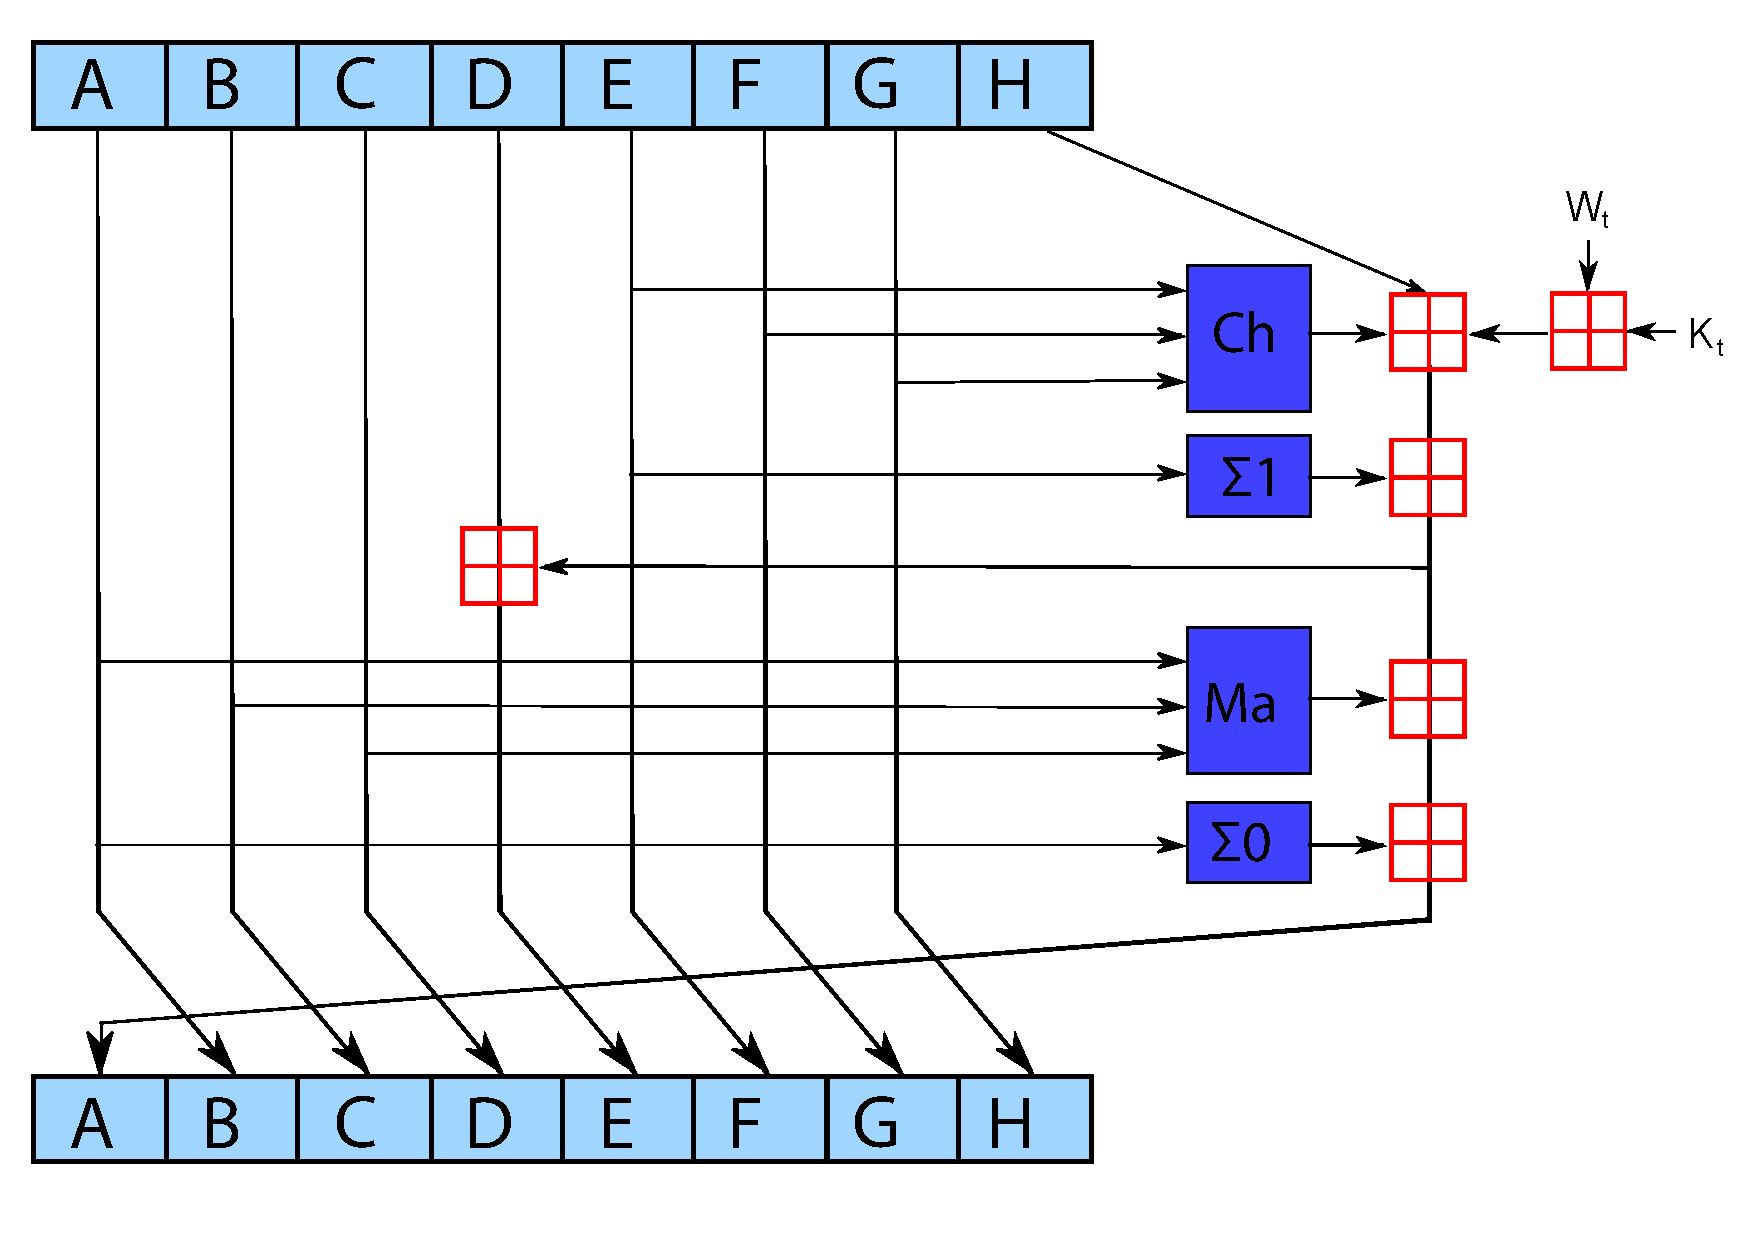
\includegraphics[scale=0.175]{res/SHA-2.pdf}
  \end{figure}
  Standard designs, like SHA, are designed over \emph{boolean fields}:
  \begin{itemize}
    \item Bitwise AND, XOR, rotation, modulo \(2^{k}\) addition\dots
    \item Extremely efficient hardware and software implementations.
    \item However, ZK-SNARKs work over prime fields \(\implies \) emulation.
    \item SHA-256 \(\approx \) \(25000\) constraints.
    \item Can we do better?
  \end{itemize}
\end{frame}

\begin{frame}{Arithmetization Oriented Primitives}
  \begin{figure}
    \centering
    
\includegraphics[scale=1.0]{res/HoevenL2019.pdf}
  \end{figure}
  \emph{Arithmetization-Oriented} (AO) cryptographic primitives:
  \begin{itemize}
    \item Build keyed permutations using prime field sum and multiplication.
    \item Apply a secure scheme to get a compression function.
    \item AO primitives can be modeled as polynomials.
    \item Must be protected against \emph{classic} and \emph{algebraic} attacks.
  \end{itemize}
\end{frame}

\begin{frame}{\Mimc{}~\cite{AlbrechtGRRT2016}}
  \begin{figure}
    \centering
    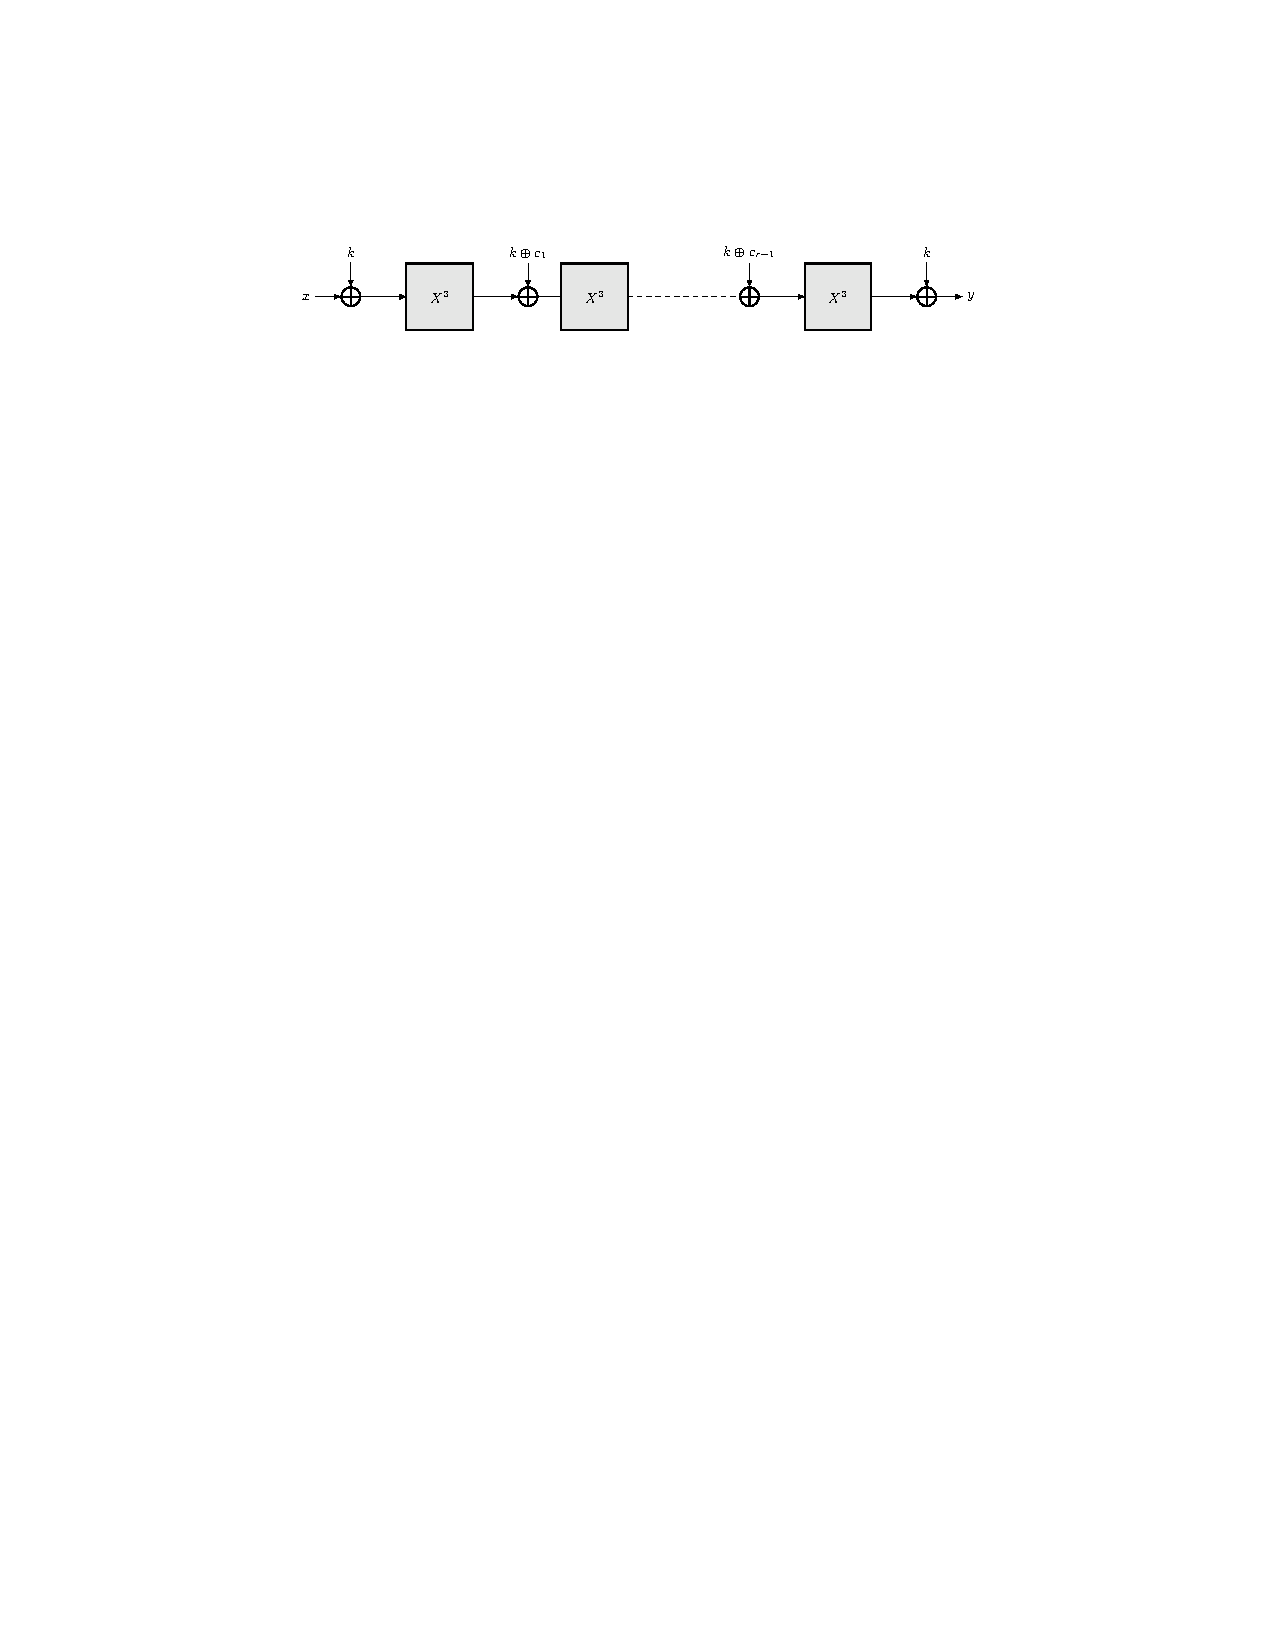
\includegraphics[scale=0.75]{res/AlbrechtGRRT2016.pdf}
  \end{figure}
  \begin{itemize}
    \item \Mimc{}: Minimal Multiplicative Complexity.
    \item Extremely simple: \emph{round function} is \(x^3 + c\).
    \item Exponent is the lowest integer in \(\mathbb{F}_p\) coprime with \(p - 1\).
    \item Many rounds to be secure against \emph{algebraic attacks}.
    \item \Mimchash-256: 640 constraints.
  \end{itemize}  
\end{frame}

\begin{frame}{\Poseidon{}~\cite{GrassiKRRS2021}}
  \begin{figure}
    \centering
    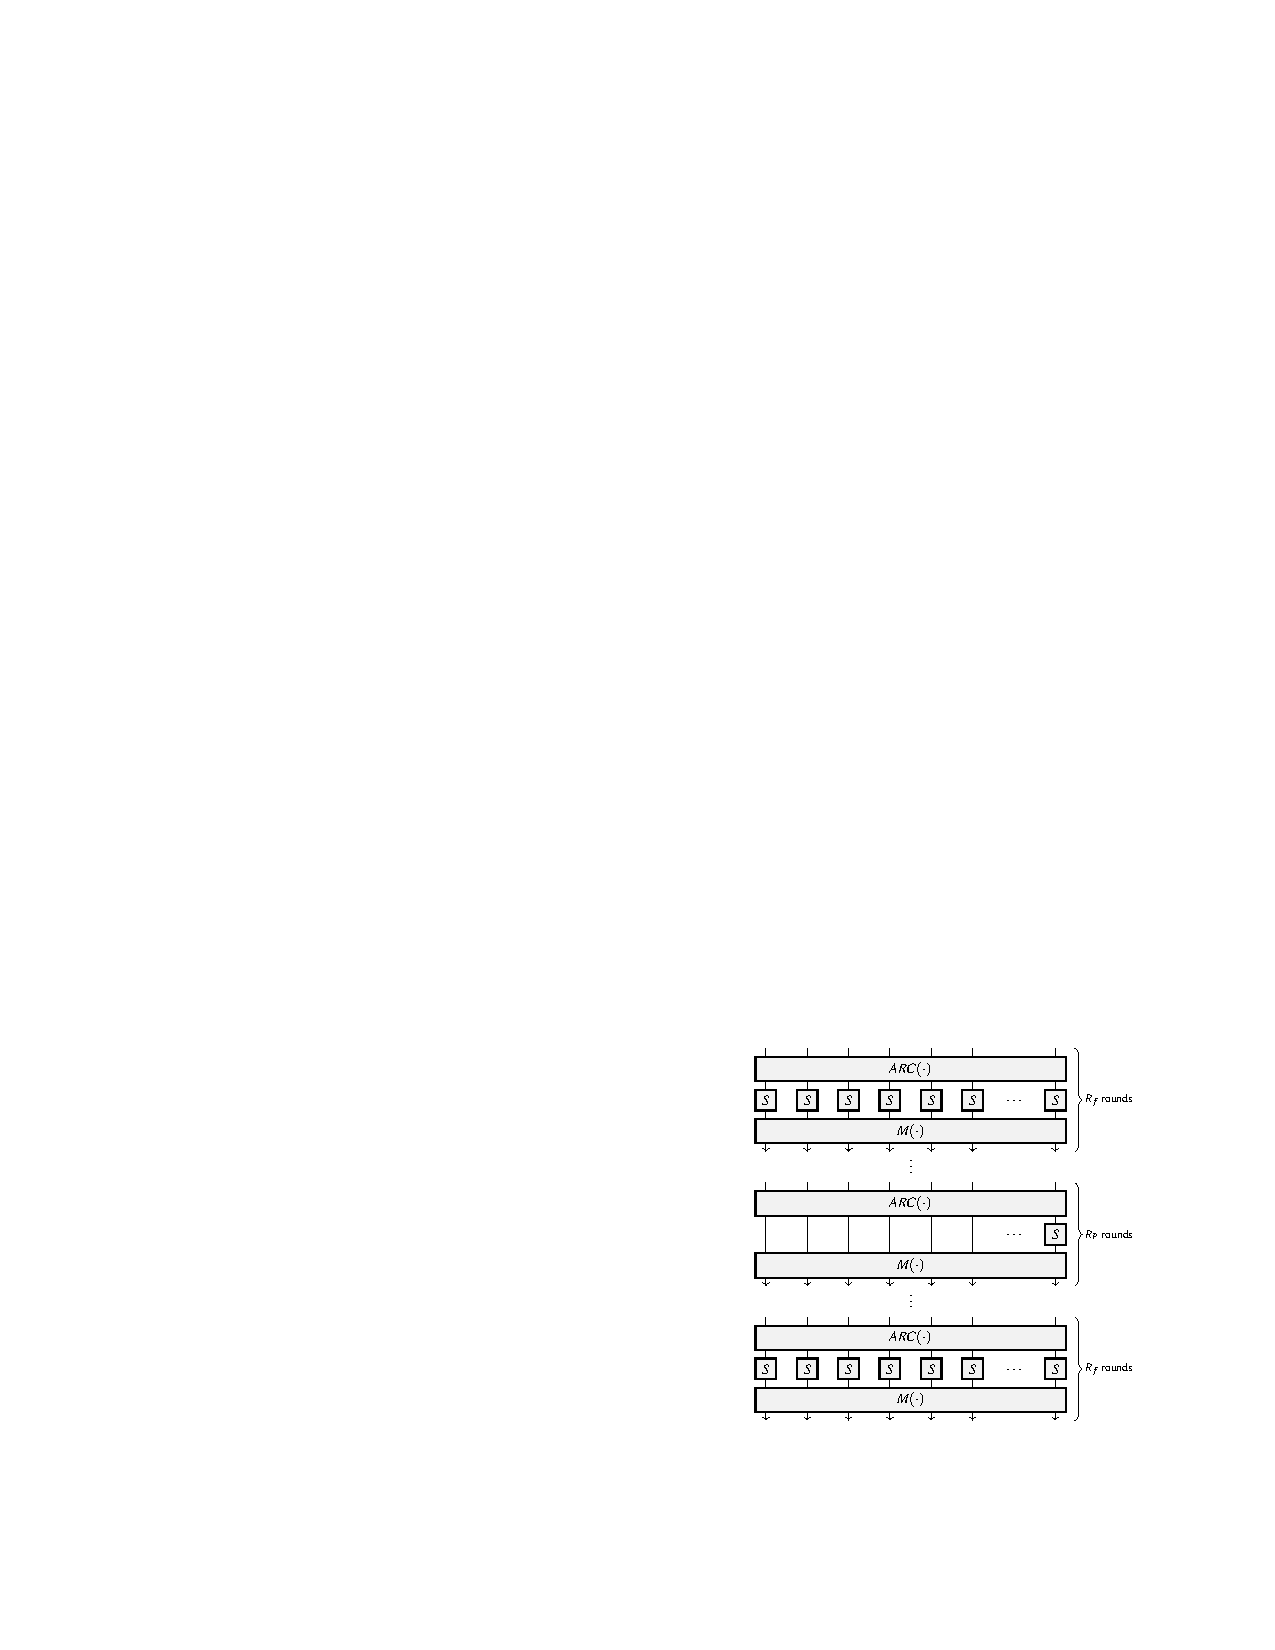
\includegraphics[scale=0.6]{res/GrassiKRRS2021.pdf}
  \end{figure}
  \begin{itemize}
    \item \Poseidon{}: Partial \emph{substitution-permutation network} (SPN).
    \item Full rounds defend against classic attacks.
    \item Partial rounds defend against algebraic attacks.
    \item \Poseidon{}-256: 240 constraints.
  \end{itemize}
\end{frame}

\begin{frame}{\Griffin{}~\cite{GrassiHRSWW2022}}
  \begin{figure}
    \centering
    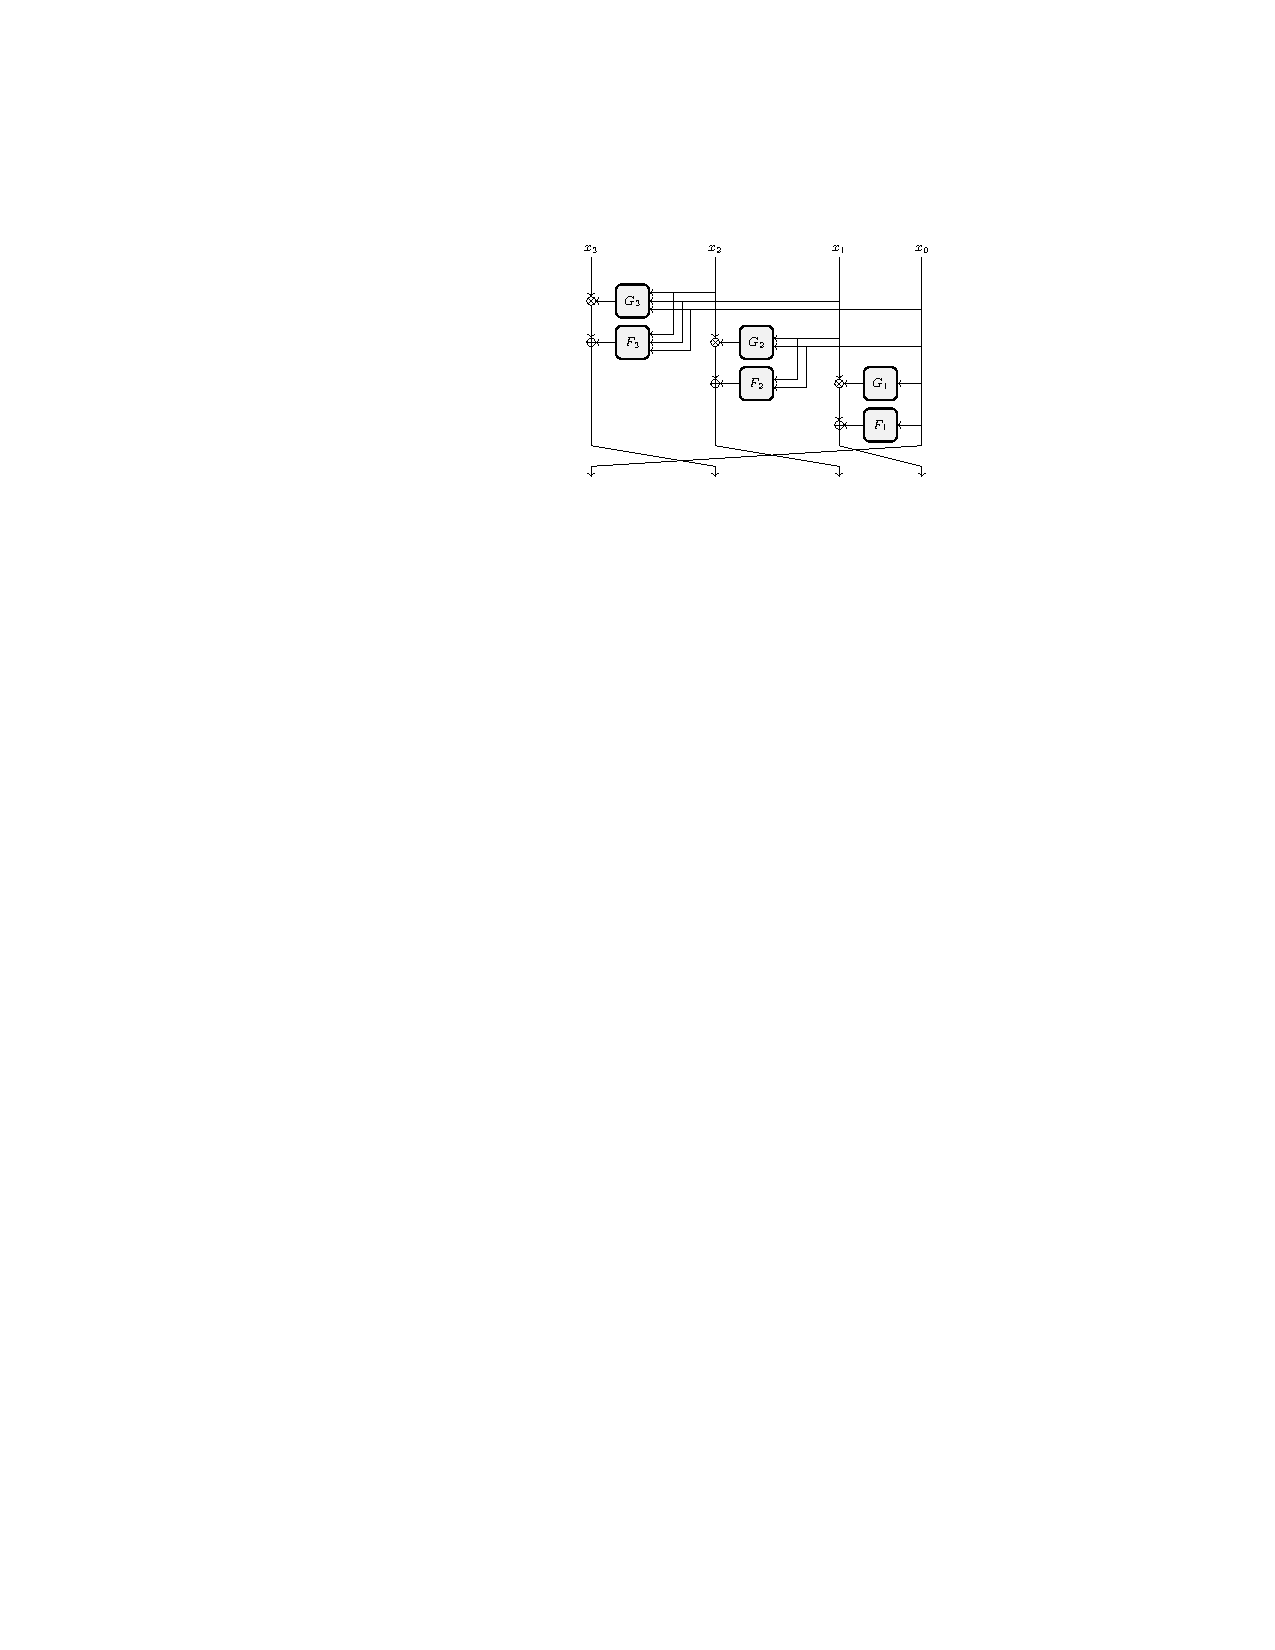
\includegraphics[scale=0.75]{res/GrassiHRSWW2022.pdf}
  \end{figure}
  \begin{itemize}
    \item \Griffin{} is based on the \Horst{} scheme: \(\Tuple{x, y} \mapsto \Tuple{y, x \otimes \call{G}{y}}\).
    \item Circulant MDS matrix in the linear layer.
    \item Inverse power to achieve faster degree growth~\cite{AlyABDS2019}.
    \item \Griffin{}-256: 96 constraints.
  \end{itemize}
\end{frame}

\begin{frame}{The GTDS~\cite{RoyS2022}}
  \begin{center}
    \begin{align*}
      & x_{1}    && \longmapsto && \call{f}{x_{n}, x_{n-1}, \dots, x_{2}, x_{1}}  \\
      & x_{2}    && \longmapsto && \call{f}{x_{n}, x_{n-1}, \dots, x_{2}}         \\
      & \cdots   && \longmapsto && \cdots                                         \\
      & x_{n-1}  && \longmapsto && \call{f}{x_{n}, x_{n-1}}                       \\
      & x_{n}    && \longmapsto && \call{f}{x_{n}}                                \\
    \end{align*}
  \end{center}

  The new \emph{Generalized Triangular Dynamical System} (GTDS):
  \begin{itemize}
    \item Includes and improves previous design strategies. 
    \item \(\begin{aligned}
        \call{f}{x_n} = y_n = x^{1/d_2}; && \call{f}{x_n, \dots, x_i} = y_i = x_i^{d_1}\call{g_i}{\sigma_{i+1}} + \call{h_i}{\sigma_{i+1}}.
    \end{aligned}\)
    \item \(\begin{aligned}
            & \sigma_{i} = \sum_{j=i}^{n}{x_j + y_j};
            && \call{g_i}{x} = x^2 + \alpha_{i}x + \beta_{i};
            && \call{h_i}{x} = x^2 + \gamma_{i}x.
          \end{aligned}\)
    \item \(\pi \)-equivalence: constraint systems unaffected by permutations.
  \end{itemize}
\end{frame}

\begin{frame}{\Arion{} and \Arionhash{}~\textbf{\cite{RoyST2023}}}
  \begin{figure}
    \centering
    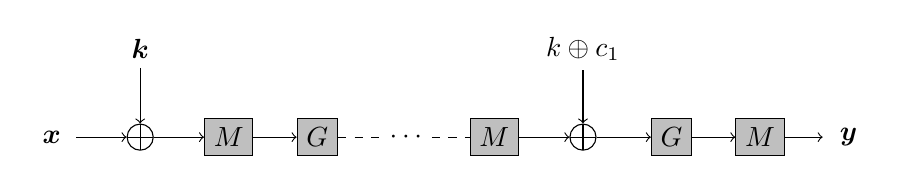
\begin{tikzpicture}[node distance={32pt}, node/.style = {draw, circle},on grid=true]
      \node[node,draw=none] (x) {\(\bm{x}\)};
      \node[xor,draw=black,fill=none] (a1) [right of=x] {};
      \node[draw=none] (c1) [above of=a1] {\(\bm{k}\)};
      \node[node,shape=rectangle,fill=lightgray] (m1) [right of=a1] {\(M\)};
      \node[node,shape=rectangle,fill=lightgray] (g1) [right of=m1] {\(G\)};
      \node (dots) [right of=g1] {\(\cdots \)};
      \node[node,shape=rectangle,fill=lightgray] (m2) [right of=dots] {\(M\)};
      \node[xor,draw=black,fill=none] (a2) [right of=m2] {};
      \node[draw=none] (c2) [above of=a2] {\(k \oplus c_1\)};
      \node[node,shape=rectangle,fill=lightgray] (g2) [right of=a2] {\(G\)};
      \node[node,shape=rectangle,fill=lightgray] (m3) [right of=g2] {\(M\)};
      \node[node,draw=none] (y) [right of=m3] {\(\bm{y}\)};

      \draw[->] (x) to (a1);
      \draw[->] (c1) to (a1);
      \draw[->] (a1) to (m1);
      \draw[->] (m1) to (g1);
      \draw[dashed,-] (g1) to (dots);
      \draw[dashed,-] (dots) to (m2);
      \draw[->] (m2) to (a2);
      \draw[->] (c2) to (a2);
      \draw[->] (a2) to (g2);
      \draw[->] (g2) to (m3);
      \draw[->] (m3) to (y);
    \end{tikzpicture}
  \end{figure}

  \Arion{}, a new keyed permutation from the GTDS\@:
  \begin{itemize}
    \item Exponent \(d_2\): easy to exponentiate by, inverse is big.
    \item Affine layer is an MDS circulant matrix easy to multiply by. 
    \item Achieves degree overflow in just one round.
    \item \Arionhash{}: OWCF based on \Arion{} in sponge mode. 
    \item \Aarionhash{}: \(76\) constraints, same guarantees as competitors.
  \end{itemize}
\end{frame}

\begin{frame}{Comparisons}
  \texttt{libsnark}: used by ZCash~\cite{SassonCGGMTV2014} for its blockchain.\\
  We used it to implement:
  \begin{itemize}
    \item Several primitives designed for ZK-SNARK, including ours.
    \item A self-parametrizing Merkle tree.
    \item A new mode of hash, the Augmented Binary tRee~\cite{AndreevaBR2021}.
  \end{itemize}
  \begin{table}
    \caption*{Proof generation times for MT commitments over 256-bit prime fields}
    \centering
        \begin{tabular}{c c c c}  
          \toprule
          Tree height & \Aarionhash{} & \Griffin{} & \Poseidon{} \\
          \midrule
          \(4\)   & \(73\) ms  & \(88\) ms & \(186\) ms  \\
          \(8\)   & \(145\) ms & \(181\) ms & \(386\) ms  \\
          \(16\)  & \(278\) ms & \(338\) ms & \(745\) ms  \\
          \(32\)  & \(509\) ms & \(622\) ms & \(1422\) ms \\
          \bottomrule
        \end{tabular}
  \end{table}
\end{frame}

\begin{frame}[allowframebreaks]  
  \bibliographystyle{alpha}
  \bibliography{biblio.bib}
\end{frame}
\end{document}
